\documentclass[8pt,a4paper,compress]{beamer}

\usepackage{/home/siyer/lib/slides}

\title{Compilation}
\date{}

\begin{document}
\begin{frame}
\vfill
\titlepage
\end{frame}

\section{Compilers}
\begin{frame}[fragile]
\pause\transdissolve

A compiler translates a high-level source language program into a low-level target language program

\begin{center}
\visible<2->{
\begin{tikzpicture}
\footnotesize
\begin{scope}[->,thin,
	   node distance=0.5cm,
  	   block1/.style={rectangle,draw,align=center},
	   block2/.style={rectangle,align=center}]
\node [block2] (1) {Source \\ Language \\ Program};
\node [block1] (2) [right=of 1] {Compiler};
\node [block2] (3) [right=of 2] {Target \\ Language \\ Program};
\path (1) edge node [above] {} (2);
\path (2) edge node [above] {} (3);
\end{scope}
\end{tikzpicture}
}
\end{center}

\pause\transdissolve\bigskip

Examples of source language: C, Java

\pause\transdissolve\bigskip

Examples of target language: MIPS instructions, JVM instructions
\end{frame}

\begin{frame}[fragile]
\pause\transdissolve

The description of a programming language consists of
\begin{itemize}
\pause\transdissolve
\item Tokens (aka lexemes)

\pause\transdissolve
\item Syntax of constructs such as classes, methods, statements and expressions

\pause\transdissolve
\item Meaning (aka semantics) of the constructs
\end{itemize}
\end{frame}

\begin{frame}[fragile]
\pause\transdissolve

A machine's instruction set and its behavior is referred to as its architecture

\pause\transdissolve\bigskip

Examples of architectures
\begin{itemize}
\pause\transdissolve
\item Intel i386: a complex instruction set computer (CISC)

\pause\transdissolve
\item MIPS: a reduced instruction set computer (RISC)

\pause\transdissolve
\item Java Virtual Machine (JVM): a virtual machine
\end{itemize}
\end{frame}

\begin{frame}[fragile]
\pause\transdissolve

An interpreter executes a high-level source language program directly

\begin{center}
\visible<2->{
\begin{tikzpicture}
\footnotesize
\begin{scope}[->,thin,
	   node distance=0.5cm,
	   block1/.style={rectangle,draw,align=center},
	   block2/.style={rectangle,align=center}]
\node [block2] (1) {Source \\ Language \\ Program};
\node [block1] (2) [right=of 1] {Interpreter};
\node [block2] (3) [right=of 2] {Results};
\path (1) edge node [above] {} (2);
\path (2) edge node [above] {} (3);
\end{scope}
\end{tikzpicture}
}
\end{center}

\pause\transdissolve\bigskip

Examples of interpreters: Bash, Python
\end{frame}

\section{Why Study Compilers?}
\begin{frame}[fragile]
\pause\transdissolve

Compilers are larger programs than the ones you have written so far

\pause\transdissolve\bigskip

Compilers make use of all those things you have learned about earlier

\pause\transdissolve\bigskip

You learn a lot about the source language (in our case, Java)

\pause\transdissolve\bigskip

You learn a lot about the target machine (in our case, JVM and MIPS)

\pause\transdissolve\bigskip

Compilers are still being written for new languages and targeted to new architectures

\pause\transdissolve\bigskip

There is a good mix of theory and practice

\pause\transdissolve\bigskip

Compiler writing is a case study in software engineering

\pause\transdissolve\bigskip

Compilers are programs and writing programs is fun
\end{frame}

\section{The Phases of Compilation}
\begin{frame}[fragile]
\pause\transdissolve

A compiler can be broken into a front end and a back end

\begin{center}
\visible<2->{
\begin{tikzpicture}
\footnotesize
\begin{scope}[->,thin,
	   node distance=0.5cm,
  	   block1/.style={rectangle,draw,align=center},
	   block2/.style={rectangle,align=center}]
\node [block2] (1) {Source \\ Language \\ Program};
\node [block1] (2) [right=of 1] {Front End};
\node [block2] (3) [right=of 2] {IR};
\node [block1] (4) [right=of 3] {Back End};
\node [block2] (5) [right=of 4] {Target \\ Language \\ Program};
\path (1) edge node [above] {} (2);
\path (2) edge node [above] {} (3);
\path (3) edge node [above] {} (4);
\path (4) edge node [above] {} (5);
\end{scope}
\end{tikzpicture}
}
\end{center}

\pause\transdissolve\bigskip

The front end analyzes the source language program for its meaning and produces an intermediate representation (IR) of the program

\pause\transdissolve\bigskip

The frond end is source language dependent and target language independent

\pause\transdissolve\bigskip

The back end takes the IR and synthesizes a target language program

\pause\transdissolve\bigskip

The back end is target language dependent and source language independent
\end{frame}

\begin{frame}[fragile]
\pause\transdissolve

The front end can be decomposed into a sequence of analysis phases

\begin{center}
\visible<2->{
\begin{tikzpicture}
\footnotesize
\begin{scope}[->,thin,
	   node distance=0.5cm,
  	   block1/.style={rectangle,draw,align=center},
	   block2/.style={rectangle,align=center}]
\node [block2] (1) {Source \\ Language \\ Program};
\node [block1] (2) [right=of 1] {Scanner};
\node [block2] (3) [right=of 2] {Tokens};
\node [block1] (4) [right=of 3] {Parser};
\node [block2] (5) [right=of 4] {AST};
\node [block1] (6) [right=of 5] {Semantics};
\node [block2] (7) [right=of 6] {IR};
\path (1) edge node [above] {} (2);
\path (2) edge node [above] {} (3);
\path (3) edge node [above] {} (4);
\path (4) edge node [above] {} (5);
\path (5) edge node [above] {} (6);
\path (6) edge node [above] {} (7);
\end{scope}
\end{tikzpicture}
}
\end{center}

\pause\transdissolve\bigskip

The scanner breaks the input stream of characters to a sequence of tokens

\pause\transdissolve\bigskip

The parser takes a sequence of tokens and parses it against a grammar to produce an abstract syntax tree (AST)

\pause\transdissolve\bigskip

The semantics phase
\begin{itemize}
\pause\transdissolve
\item Declares names in a symbol table

\pause\transdissolve
\item Looks up names as they are referenced to determine their types 

\pause\transdissolve
\item Assigns types to expressions and checks the validity of types

\pause\transdissolve
\item Does certain amount of storage analysis 
\end{itemize}
\end{frame}

\begin{frame}[fragile]
\pause\transdissolve

The back end can be decomposed into a sequence of synthesis phases

\begin{center}
\visible<2->{
\begin{tikzpicture}
\footnotesize
\begin{scope}[->,thin,
	   node distance=0.5cm,
  	   block1/.style={rectangle,draw,align=center},
	   block2/.style={rectangle,align=center}]
\node [block2] (1) {IR};
\node [block1] (2) [right=of 1] {Codegen};
\node [block2] (3) [right=of 2] {Target \\ Language \\ Instructions};
\node [block1] (4) [right=of 3] {Peephole};
\node [block2] (5) [right=of 4] {Better \\ Target \\ Language \\ Instructions};
\node [block1] (6) [right=of 5] {Object};
\node [block2] (7) [right=of 6] {Target \\ Language \\ Program};
\path (1) edge node [above] {} (2);
\path (2) edge node [above] {} (3);
\path (3) edge node [above] {} (4);
\path (4) edge node [above] {} (5);
\path (5) edge node [above] {} (6);
\path (6) edge node [above] {} (7);
\end{scope}
\end{tikzpicture}
}
\end{center}

\pause\transdissolve\bigskip

The code generation phase chooses what target machine instructions to generate

\pause\transdissolve\bigskip

The peephole phase scans through the generated instructions locally for wasteful instructions such as branches to branches and unnecessary load/store pairs

\pause\transdissolve\bigskip

The object phase links together modules produced in code generation and constructs a single target language program
\end{frame}

\begin{frame}[fragile]
\pause\transdissolve

A compiler sometimes has an optimizer between the front end and the back end

\begin{center}
\visible<2->{
\begin{tikzpicture}
\footnotesize
\begin{scope}[->,thin,
	   node distance=0.5cm,
  	   block1/.style={rectangle,draw,align=center},
	   block2/.style={rectangle,align=center}]
\node [block2] (1) {Source \\ Language \\ Program};
\node [block1] (2) [right=of 1] {Front End};
\node [block2] (3) [right=of 2] {IR};
\node [block1] (4) [right=of 3] {Optimizer};
\node [block2] (5) [right=of 4] {IR};
\node [block1] (6) [right=of 5] {Back End};
\node [block2] (7) [right=of 6] {Target \\ Language \\ Program};
\path (1) edge node [above] {} (2);
\path (2) edge node [above] {} (3);
\path (3) edge node [above] {} (4);
\path (4) edge node [above] {} (5);
\path (5) edge node [above] {} (6);
\path (6) edge node [above] {} (7);
\end{scope}
\end{tikzpicture}
}
\end{center}

\pause\transdissolve\bigskip

The optimizer might
\begin{itemize}
\pause\transdissolve
\item Eliminate common sub-expressions

\pause\transdissolve
\item Perform constant folding

\pause\transdissolve
\item Lift loop invariants out of loops

\pause\transdissolve
\item Perform strength reduction
\end{itemize}
\end{frame}

\begin{frame}[fragile]
\pause\transdissolve

Advantages of separating the front end from the back end
\begin{itemize}
\pause\transdissolve
\item It is easier to understand (and implement) smaller programs

\pause\transdissolve
\item Several individuals or teams can work concurrently on separate parts

\pause\transdissolve
\item Enables a certain amount of code re-use

\bigskip
\begin{minipage}[t]{\linewidth}
\begin{center}
\begin{overprint}
\onslide<6>
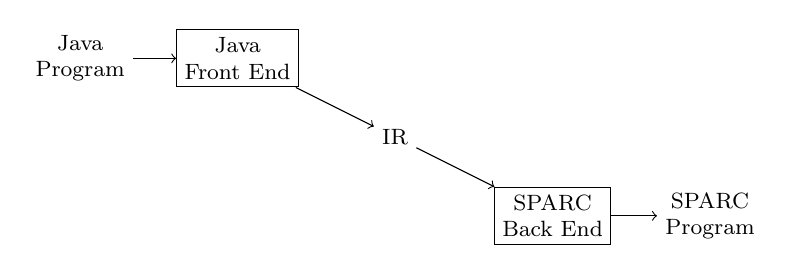
\begin{tikzpicture}
\footnotesize
\begin{scope}[->,thin,
              block1/.style={rectangle,draw,align=center},
	          block2/.style={rectangle,align=center}]
    \node [block2] (1) at (0,2) {Java \\ Program};
%    \node [block2] (2) at (0,0) {C \\ Program};
    \node [block1] (3) at (2,2) {Java \\ Front End};
%    \node [block1] (4) at (2,0) {C \\ Front End};
%    \node [block1] (5) at (6,2) {Intel \\ Back End};
    \node [block1] (6) at (6,0) {SPARC \\ Back End};
%    \node [block2] (7) at (8,2) {Intel Core Duo \\ Program};
    \node [block2] (8) at (8,0) {SPARC \\ Program};
    \node [block2] (9) at (4,1) {IR};
    \path (1) edge node [above] {} (3);
%    \path (2) edge node [above] {} (4);
%    \path (5) edge node [above] {} (7);
    \path (6) edge node [above] {} (8);
    \path (3) edge node [above] {} (9);
%    \path (4) edge node [above] {} (9);
%    \path (9) edge node [above] {} (5);
    \path (9) edge node [above] {} (6);
\end{scope}
\end{tikzpicture}

\onslide<7>
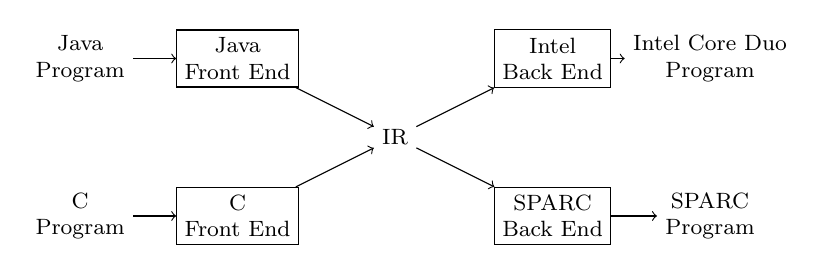
\begin{tikzpicture}
\footnotesize
\begin{scope}[->,thin,
              block1/.style={rectangle,draw,align=center},
	          block2/.style={rectangle,align=center}]
    \node [block2] (1) at (0,2) {Java \\ Program};
    \node [block2] (2) at (0,0) {C \\ Program};
    \node [block1] (3) at (2,2) {Java \\ Front End};
    \node [block1] (4) at (2,0) {C \\ Front End};
    \node [block1] (5) at (6,2) {Intel \\ Back End};
    \node [block1] (6) at (6,0) {SPARC \\ Back End};
    \node [block2] (7) at (8,2) {Intel Core Duo \\ Program};
    \node [block2] (8) at (8,0) {SPARC \\ Program};
    \node [block2] (9) at (4,1) {IR};
    \path (1) edge node [above] {} (3);
    \path (2) edge node [above] {} (4);
    \path (5) edge node [above] {} (7);
    \path (6) edge node [above] {} (8);
    \path (3) edge node [above] {} (9);
    \path (4) edge node [above] {} (9);
    \path (9) edge node [above] {} (5);
    \path (9) edge node [above] {} (6);
\end{scope}
\end{tikzpicture} 
\end{overprint}
\end{center}
\end{minipage}
\end{itemize}
\end{frame}

\begin{frame}[fragile]
\pause\transdissolve

We will implement a compiler called \jmm to compile a non-trivial subset of Java, also called \jmm

\pause\transdissolve\bigskip

In the first instance, we will target the JVM, a stack-based architecture

\pause\transdissolve\bigskip

Compiling a \jmm program \lstinline{P.java} for JVM
\begin{tcolorbox}[enhanced,drop shadow southwest,sharp corners,size=fbox,colback=black]
\begin{lstlisting}[style=terminal]
$ j-- P.java
\end{lstlisting}
\end{tcolorbox}

\pause\transdissolve\bigskip

Running the JVM program \lstinline{P.class}
\begin{tcolorbox}[enhanced,drop shadow southwest,sharp corners,size=fbox,colback=black]
\begin{lstlisting}[style=terminal]
$ java P
\end{lstlisting}
\end{tcolorbox}

\pause\transdissolve\bigskip

In the second instance, we will target the MIPS machine, a register-based architecture

\pause\transdissolve\bigskip

Compiling a \jmm program \lstinline{P.java} for MIPS
\begin{tcolorbox}[enhanced,drop shadow southwest,sharp corners,size=fbox,colback=black]
\begin{lstlisting}[style=terminal]
$ j-- -s naive P.java
\end{lstlisting}
\end{tcolorbox}

\pause\transdissolve\bigskip

Running the MIPS program \lstinline{P.s}

\begin{tcolorbox}[enhanced,drop shadow southwest,sharp corners,size=fbox,colback=black]
\begin{lstlisting}[style=terminal]
$ spim -f P.s
\end{lstlisting}
\end{tcolorbox}
\end{frame}

\section{Overview of the \protect \jmm to JVM Compiler}
\begin{frame}[fragile]
\pause\transdissolve

\jmm is an object-oriented programming language, supporting classes, methods, fields, message expressions, and a variety of statements, expressions and primitive types

\pause\transdissolve\bigskip

The \jmm compiler is organized in an object-oriented fashion

\bigskip

\begin{center}
\begin{overprint}
\onslide<4>
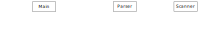
\includegraphics[scale=0.45]{figures/organization1.pdf}

\onslide<5>
\includegraphics[scale=0.45]{figures/organization2.pdf}

\onslide<6>
\includegraphics[scale=0.45]{figures/organization3.pdf}

\onslide<7>
\includegraphics[scale=0.45]{figures/organization4.pdf}

\onslide<8>
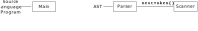
\includegraphics[scale=0.45]{figures/organization5.pdf}

\onslide<9>
\includegraphics[scale=0.45]{figures/organization6.pdf}

\onslide<10>
\includegraphics[scale=0.45]{figures/organization7.pdf}

\onslide<11>
\includegraphics[scale=0.45]{figures/organization8.pdf}

\onslide<12>
\includegraphics[scale=0.45]{figures/organization9.pdf}
\end{overprint}
\end{center}
\end{frame}

\begin{frame}[fragile]
\pause\transdissolve

The scanner breaks down a \jmm program into a sequence of tokens

\pause\transdissolve\bigskip

For example, consider the program

\pause\transdissolve\smallskip

\begin{tcolorbox}[enhanced,drop shadow southwest,sharp corners,size=fbox,colback=white,fontlower=\small\ttfamily,collower=silver100]

\begin{lstlisting}[language=Java,style=focusin]
import java.lang.System;

public class HelloWorld {
    // The only method.
    public static void main(String[] args) {
        System.out.println("Hello, World!");
    }
}
\end{lstlisting}
\end{tcolorbox}

\pause\transdissolve\smallskip

The program is broken down into tokens \lstinline{import}, \lstinline{java}, \lstinline{.}, \lstinline{lang}, \lstinline{.}, \lstinline{System}, \lstinline{;}, and so on

\pause\transdissolve\bigskip

Tokens such as \lstinline{java} and \lstinline{HelloWorld} are \lstinline{IDENTIFIER} tokens, carrying along their images (\lstinline{"java"} and \lstinline{"HelloWorld"}) as attributes

\pause\transdissolve\bigskip

Tokens such as \lstinline{import} and \lstinline{public} are reserved words having the unique names such as \lstinline{IMPORT} and \lstinline{PUBLIC}

\pause\transdissolve\bigskip

Operators and separators such as \lstinline{+} and \lstinline{;} have distinct names such as \lstinline{PLUS} and \lstinline{SEMI}

\pause\transdissolve\bigskip

Literals such as \lstinline{"Hello, World!"} comprise a single token such as \lstinline{STRING_LITERAL}

\pause\transdissolve\bigskip

Comments are scanned and ignored altogether
\end{frame}

\begin{frame}[fragile]
\pause\transdissolve

The parser validates the syntax of a \jmm program against the \jmm grammar and represents the program as an AST

\pause\transdissolve\bigskip

In the first instance, the parser is hand-crafted from the grammar, to parse programs by a technique known as recursive descent

\pause\transdissolve\bigskip

For example, consider the grammar rule describing a compilation unit

\pause\transdissolve\smallskip

\begin{overprint}
\onslide<5>
\begin{tcolorbox}[enhanced,drop shadow southwest,sharp corners,size=fbox,colback=white,fontlower=\small\ttfamily,collower=silver900]

\begin{lstlisting}[language={},style=focusin]
compilationUnit ::= [PACKAGE qualifiedIdentifier SEMI]
                    {IMPORT  qualifiedIdentifier SEMI}
                    {typeDeclaration} 
                    EOF
\end{lstlisting}

\tcblower
\begin{minipage}[t][.25cm][t]{\textwidth}

\end{minipage}
\end{tcolorbox}

\onslide<6>
\begin{tcolorbox}[enhanced,drop shadow southwest,sharp corners,size=fbox,colback=white,fontlower=\small\ttfamily,collower=silver900]

\begin{lstlisting}[language={},style=focusin,backgroundcolor=\color{lime100}]
compilationUnit ::= [PACKAGE qualifiedIdentifier SEMI]
\end{lstlisting}
\begin{lstlisting}[language={},style=focusout]
                    {IMPORT  qualifiedIdentifier SEMI}
                    {typeDeclaration} 
                    EOF
\end{lstlisting}

\tcblower
\begin{minipage}[t][.25cm][t]{\textwidth}
optional package statement
\end{minipage}
\end{tcolorbox}

\onslide<7>
\begin{tcolorbox}[enhanced,drop shadow southwest,sharp corners,size=fbox,colback=white,fontlower=\small\ttfamily,collower=silver900]

\begin{lstlisting}[language={},style=focusout]
compilationUnit ::= [PACKAGE qualifiedIdentifier SEMI]
\end{lstlisting}
\begin{lstlisting}[language={},style=focusin,backgroundcolor=\color{lime100}]
                    {IMPORT  qualifiedIdentifier SEMI}
\end{lstlisting}
\begin{lstlisting}[language={},style=focusout]
                    {typeDeclaration} 
                    EOF
\end{lstlisting}

\tcblower
\begin{minipage}[t][.25cm][t]{\textwidth}
zero or more import statements
\end{minipage}
\end{tcolorbox}

\onslide<8>
\begin{tcolorbox}[enhanced,drop shadow southwest,sharp corners,size=fbox,colback=white,fontlower=\small\ttfamily,collower=silver900]

\begin{lstlisting}[language={},style=focusout]
compilationUnit ::= [PACKAGE qualifiedIdentifier SEMI]
                    {IMPORT  qualifiedIdentifier SEMI}
\end{lstlisting}
\begin{lstlisting}[language={},style=focusin,backgroundcolor=\color{lime100}]
                    {typeDeclaration} 
\end{lstlisting}
\begin{lstlisting}[language={},style=focusout]
                    EOF
\end{lstlisting}
\tcblower
\begin{minipage}[t][.25cm][t]{\textwidth}
zero or more type (class) declarations
\end{minipage}
\end{tcolorbox}

\onslide<9>
\begin{tcolorbox}[enhanced,drop shadow southwest,sharp corners,size=fbox,colback=white,fontlower=\small\ttfamily,collower=silver900]

\begin{lstlisting}[language={},style=focusout]
compilationUnit ::= [PACKAGE qualifiedIdentifier SEMI]
                    {IMPORT  qualifiedIdentifier SEMI}
                    {typeDeclaration} 
\end{lstlisting}
\begin{lstlisting}[language={},style=focusin,backgroundcolor=\color{lime100}]
                    EOF
\end{lstlisting}

\tcblower
\begin{minipage}[t][.25cm][t]{\textwidth}
end of file
\end{minipage}
\end{tcolorbox}

\onslide<10>

\begin{tcolorbox}[enhanced,drop shadow southwest,sharp corners,size=fbox,colback=white,fontlower=\small\ttfamily,collower=silver900]

\begin{lstlisting}[language={},style=focusin]
compilationUnit ::= [PACKAGE qualifiedIdentifier SEMI]
                    {IMPORT  qualifiedIdentifier SEMI}
                    {typeDeclaration} 
                    EOF
\end{lstlisting}

\tcblower
\begin{minipage}[t][.25cm][t]{\textwidth}

\end{minipage}
\end{tcolorbox}

\onslide<11>

\begin{tcolorbox}[enhanced,drop shadow southwest,sharp corners,size=fbox,colback=white,fontlower=\small\ttfamily,collower=silver900]

\begin{lstlisting}[language={},style=focusin]
compilationUnit ::= [PACKAGE qualifiedIdentifier SEMI]
                    {IMPORT  qualifiedIdentifier SEMI}
                    {typeDeclaration} 
                    EOF
\end{lstlisting}

\tcblower
\begin{minipage}[t][.25cm][t]{\textwidth}

\end{minipage}
\end{tcolorbox}

The rule is handled by the method \lstinline{compilationUnit()} defined in \lstinline{Parser.java} (the hand-crafted parser)
\end{overprint}
\end{frame}

\begin{frame}[fragile]
\pause\transdissolve

\begin{tcolorbox}[enhanced,drop shadow southwest,sharp corners,size=fbox,colback=white,fontlower=\small\ttfamily,collower=silver900]

\begin{lstlisting}[language=Java,style=focusin]
    public JCompilationUnit compilationUnit() {
        int line = scanner.token().line();
        TypeName packageName = null;
        if (have(PACKAGE)) {
            packageName = qualifiedIdentifier();
            mustBe(SEMI);
        }
        ArrayList<TypeName> imports = new ArrayList<TypeName>();
        while (have(IMPORT)) {
            imports.add(qualifiedIdentifier());
            mustBe(SEMI);
        }
        ArrayList<JAST> typeDeclarations = new ArrayList<JAST>();
        while (!see(EOF)) {
            JAST typeDeclaration = typeDeclaration();
            if (typeDeclaration != null) {
                typeDeclarations.add(typeDeclaration);
            }
        }
        mustBe(EOF);
        return new JCompilationUnit(scanner.fileName(), line, 
            packageName, imports, typeDeclarations);
    }
\end{lstlisting}

\tcblower
\begin{minipage}[t][.25cm][t]{\textwidth}

\end{minipage}
\end{tcolorbox}
\end{frame}

\begin{frame}[fragile]
\transdissolve

\begin{tcolorbox}[enhanced,drop shadow southwest,sharp corners,size=fbox,colback=white,fontlower=\small\ttfamily,collower=silver900]

\begin{lstlisting}[language=Java,style=focusin,backgroundcolor=\color{lime100}]
    public JCompilationUnit compilationUnit() {
\end{lstlisting}
\begin{lstlisting}[language=Java,style=focusout]
        int line = scanner.token().line();
        TypeName packageName = null;
        if (have(PACKAGE)) {
            packageName = qualifiedIdentifier();
            mustBe(SEMI);
        }
        ArrayList<TypeName> imports = new ArrayList<TypeName>();
        while (have(IMPORT)) {
            imports.add(qualifiedIdentifier());
            mustBe(SEMI);
        }
        ArrayList<JAST> typeDeclarations = new ArrayList<JAST>();
        while (!see(EOF)) {
            JAST typeDeclaration = typeDeclaration();
            if (typeDeclaration != null) {
                typeDeclarations.add(typeDeclaration);
            }
        }
        mustBe(EOF);
        return new JCompilationUnit(scanner.fileName(), line, 
            packageName, imports, typeDeclarations);
    }
\end{lstlisting}

\tcblower
\begin{minipage}[t][.25cm][t]{\textwidth}
parse a compilation unit and return an AST representation for it
\end{minipage}
\end{tcolorbox}
\end{frame}

\begin{frame}[fragile]
\transdissolve

\begin{tcolorbox}[enhanced,drop shadow southwest,sharp corners,size=fbox,colback=white,fontlower=\small\ttfamily,collower=silver900]

\begin{lstlisting}[language=Java,style=focusout]
    public JCompilationUnit compilationUnit() {
\end{lstlisting}
\begin{lstlisting}[language=Java,style=focusin,backgroundcolor=\color{lime100}]
        int line = scanner.token().line();
\end{lstlisting}
\begin{lstlisting}[language=Java,style=focusout]
        TypeName packageName = null;
        if (have(PACKAGE)) {
            packageName = qualifiedIdentifier();
            mustBe(SEMI);
        }
        ArrayList<TypeName> imports = new ArrayList<TypeName>();
        while (have(IMPORT)) {
            imports.add(qualifiedIdentifier());
            mustBe(SEMI);
        }
        ArrayList<JAST> typeDeclarations = new ArrayList<JAST>();
        while (!see(EOF)) {
            JAST typeDeclaration = typeDeclaration();
            if (typeDeclaration != null) {
                typeDeclarations.add(typeDeclaration);
            }
        }
        mustBe(EOF);
        return new JCompilationUnit(scanner.fileName(), line, 
            packageName, imports, typeDeclarations);
    }
\end{lstlisting}

\tcblower
\begin{minipage}[t][.25cm][t]{\textwidth}
get line number of current token
\end{minipage}
\end{tcolorbox}
\end{frame}

\begin{frame}[fragile]
\transdissolve

\begin{tcolorbox}[enhanced,drop shadow southwest,sharp corners,size=fbox,colback=white,fontlower=\small\ttfamily,collower=silver900]

\begin{lstlisting}[language=Java,style=focusout]
    public JCompilationUnit compilationUnit() {
        int line = scanner.token().line();
\end{lstlisting}
\begin{lstlisting}[language=Java,style=focusin,backgroundcolor=\color{lime100}]
        TypeName packageName = null;
        if (have(PACKAGE)) {
            packageName = qualifiedIdentifier();
            mustBe(SEMI);
        }
\end{lstlisting}
\begin{lstlisting}[language=Java,style=focusout]
        ArrayList<TypeName> imports = new ArrayList<TypeName>();
        while (have(IMPORT)) {
            imports.add(qualifiedIdentifier());
            mustBe(SEMI);
        }
        ArrayList<JAST> typeDeclarations = new ArrayList<JAST>();
        while (!see(EOF)) {
            JAST typeDeclaration = typeDeclaration();
            if (typeDeclaration != null) {
                typeDeclarations.add(typeDeclaration);
            }
        }
        mustBe(EOF);
        return new JCompilationUnit(scanner.fileName(), line, 
            packageName, imports, typeDeclarations);
    }
\end{lstlisting}

\tcblower
\begin{minipage}[t][.25cm][t]{\textwidth}
parse optional package statement
\end{minipage}
\end{tcolorbox}
\end{frame}

\begin{frame}[fragile]
\transdissolve

\begin{tcolorbox}[enhanced,drop shadow southwest,sharp corners,size=fbox,colback=white,fontlower=\small\ttfamily,collower=silver900]

\begin{lstlisting}[language=Java,style=focusout]
    public JCompilationUnit compilationUnit() {
        int line = scanner.token().line();
        TypeName packageName = null;
        if (have(PACKAGE)) {
            packageName = qualifiedIdentifier();
            mustBe(SEMI);
        }
\end{lstlisting}
\begin{lstlisting}[language=Java,style=focusin,backgroundcolor=\color{lime100}]
        ArrayList<TypeName> imports = new ArrayList<TypeName>();
        while (have(IMPORT)) {
            imports.add(qualifiedIdentifier());
            mustBe(SEMI);
        }
\end{lstlisting}
\begin{lstlisting}[language=Java,style=focusout]
        ArrayList<JAST> typeDeclarations = new ArrayList<JAST>();
        while (!see(EOF)) {
            JAST typeDeclaration = typeDeclaration();
            if (typeDeclaration != null) {
                typeDeclarations.add(typeDeclaration);
            }
        }
        mustBe(EOF);
        return new JCompilationUnit(scanner.fileName(), line, 
            packageName, imports, typeDeclarations);
    }
\end{lstlisting}

\tcblower
\begin{minipage}[t][.25cm][t]{\textwidth}
parse zero or more import statements
\end{minipage}
\end{tcolorbox}
\end{frame}

\begin{frame}[fragile]
\transdissolve

\begin{tcolorbox}[enhanced,drop shadow southwest,sharp corners,size=fbox,colback=white,fontlower=\small\ttfamily,collower=silver900]

\begin{lstlisting}[language=Java,style=focusout]
    public JCompilationUnit compilationUnit() {
        int line = scanner.token().line();
        TypeName packageName = null;
        if (have(PACKAGE)) {
            packageName = qualifiedIdentifier();
            mustBe(SEMI);
        }
        ArrayList<TypeName> imports = new ArrayList<TypeName>();
        while (have(IMPORT)) {
            imports.add(qualifiedIdentifier());
            mustBe(SEMI);
        }
\end{lstlisting}
\begin{lstlisting}[language=Java,style=focusin,backgroundcolor=\color{lime100}]
        ArrayList<JAST> typeDeclarations = new ArrayList<JAST>();
        while (!see(EOF)) {
            JAST typeDeclaration = typeDeclaration();
            if (typeDeclaration != null) {
                typeDeclarations.add(typeDeclaration);
            }
        }
\end{lstlisting}
\begin{lstlisting}[language=Java,style=focusout]
        mustBe(EOF);
        return new JCompilationUnit(scanner.fileName(), line, 
            packageName, imports, typeDeclarations);
    }
\end{lstlisting}

\tcblower
\begin{minipage}[t][.25cm][t]{\textwidth}
parse zero or more type (class) declarations
\end{minipage}
\end{tcolorbox}
\end{frame}

\begin{frame}[fragile]
\transdissolve

\begin{tcolorbox}[enhanced,drop shadow southwest,sharp corners,size=fbox,colback=white,fontlower=\small\ttfamily,collower=silver900]

\begin{lstlisting}[language=Java,style=focusout]
    public JCompilationUnit compilationUnit() {
        int line = scanner.token().line();
        TypeName packageName = null;
        if (have(PACKAGE)) {
            packageName = qualifiedIdentifier();
            mustBe(SEMI);
        }
        ArrayList<TypeName> imports = new ArrayList<TypeName>();
        while (have(IMPORT)) {
            imports.add(qualifiedIdentifier());
            mustBe(SEMI);
        }
        ArrayList<JAST> typeDeclarations = new ArrayList<JAST>();
        while (!see(EOF)) {
            JAST typeDeclaration = typeDeclaration();
            if (typeDeclaration != null) {
                typeDeclarations.add(typeDeclaration);
            }
        }
\end{lstlisting}
\begin{lstlisting}[language=Java,style=focusin,backgroundcolor=\color{lime100}]
        mustBe(EOF);
\end{lstlisting}
\begin{lstlisting}[language=Java,style=focusout]
        return new JCompilationUnit(scanner.fileName(), line, 
            packageName, imports, typeDeclarations);
    }
\end{lstlisting}

\tcblower
\begin{minipage}[t][.25cm][t]{\textwidth}
parse end of file
\end{minipage}
\end{tcolorbox}
\end{frame}

\begin{frame}[fragile]
\transdissolve

\begin{tcolorbox}[enhanced,drop shadow southwest,sharp corners,size=fbox,colback=white,fontlower=\small\ttfamily,collower=silver900]

\begin{lstlisting}[language=Java,style=focusout]
    public JCompilationUnit compilationUnit() {
        int line = scanner.token().line();
        TypeName packageName = null;
        if (have(PACKAGE)) {
            packageName = qualifiedIdentifier();
            mustBe(SEMI);
        }
        ArrayList<TypeName> imports = new ArrayList<TypeName>();
        while (have(IMPORT)) {
            imports.add(qualifiedIdentifier());
            mustBe(SEMI);
        }
        ArrayList<JAST> typeDeclarations = new ArrayList<JAST>();
        while (!see(EOF)) {
            JAST typeDeclaration = typeDeclaration();
            if (typeDeclaration != null) {
                typeDeclarations.add(typeDeclaration);
            }
        }
        mustBe(EOF);
\end{lstlisting}
\begin{lstlisting}[language=Java,style=focusin,backgroundcolor=\color{lime100}]
        return new JCompilationUnit(scanner.fileName(), line, 
            packageName, imports, typeDeclarations);
\end{lstlisting}
\begin{lstlisting}[language=Java,style=focusout]
    }
\end{lstlisting}

\tcblower
\begin{minipage}[t][.25cm][t]{\textwidth}
return an AST representation for the compilation unit
\end{minipage}
\end{tcolorbox}
\end{frame}

\begin{frame}[fragile]
\pause\transdissolve

\jmm (like Java) is statically typed, so it must determine the types of all names and expressions

\pause\transdissolve\bigskip

Types in \jmm are represented using
\begin{itemize}
\pause\transdissolve
\item \lstinline{Type} (wraps \lstinline{java.lang.Class})

\pause\transdissolve
\item \lstinline{Method} (wraps \lstinline{java.lang.reflect.Method})

\pause\transdissolve
\item \lstinline{Constructor} (wraps \lstinline{java.lang.reflect.Constructor})

\pause\transdissolve
\item \lstinline{Field} (wraps \lstinline{java.lang.reflect.Field})

\pause\transdissolve
\item \lstinline{Member} (wraps \lstinline{java.lang.reflect.Member})
\end{itemize}

\pause\transdissolve\bigskip

There are places where \jmm uses \lstinline{TypeName} and \lstinline{ArrayTypeName} to denote a type by its name, before the type is known or defined
\end{frame}

\begin{frame}[fragile]
\pause\transdissolve

\jmm maintains a symbol table (a singly-linked list of \lstinline{Context} objects) in which it declares names

\pause\transdissolve\bigskip

Each object in the symbol table represents some area of scope and contains a mapping from names to definitions

\pause\transdissolve\bigskip

A \lstinline{CompilationUnitContext} object represents the scope comprising the program

\pause\transdissolve\bigskip

A \lstinline{ClassContext} object represents the scope of a class declaration

\pause\transdissolve\bigskip

A \lstinline{LocalContext} object represents the scope of a block

\pause\transdissolve\bigskip

A \lstinline{MethodContext} (subclass of \lstinline{LocalContext}) object represents the scopes of methods and constructors
\end{frame}

\begin{frame}[fragile]
\pause\transdissolve

\lstinline{preAnalyze()} builds the part of the symbol table that is close to the top of the AST, declaring imported types, types introduced by class declarations, and the members in those classes

\pause\transdissolve\bigskip

\lstinline{analyze()} builds the rest of the symbol table, decorating the AST with type information

\pause\transdissolve\bigskip

\lstinline{analyze()} also performs other important tasks such as type checking, accessibility checking, member finding, tree rewriting, and storage allocation
\end{frame}

\begin{frame}[fragile]
\pause

The JVM is a stack machine: all computations are carried out atop the run-time stack

\pause
\bigskip

Each time a method is invoked, the JVM allocates a stack frame, a contiguous block of
memory locations on top of the run-time stack; the actual arguments substituted for formal parameters, the values of local variables, and temporary results are all given positions within this stack frame

\begin{center}
\visible<3->{\includegraphics[scale=0.5]{{figures/figure01.10}.jpg}}
\end{center}
\end{frame}

\begin{frame}[fragile]
\pause

The purpose of \lstinline{codegen()} is to generate JVM byte code from the AST, based on information computed by \lstinline{preAnalyze()} and \lstinline{analyze()}

\pause
\bigskip

\lstinline{codegen()} is invoked by \lstinline{Main} on the root of the AST, and \lstinline{codegen()} recursively descends the AST, generating byte code

\pause
\bigskip

\lstinline{CLEmitter} provides an abstraction for the JVM class file, hiding many of the gory details

\pause
\bigskip

Here's the implementation of \lstinline{codegen()} in \lstinline{JMethodDeclaration} (AST representation for method declarations)

\begin{lstlisting}[language=Java]
    public void codegen(CLEmitter output) {
        output.addMethod(mods, name, descriptor, null, false);
        if (body != null) {
            body.codegen(output);
        }

        // Add implicit RETURN
        if (returnType == Type.VOID) {
            output.addNoArgInstruction(RETURN);
        }
    }
\end{lstlisting}
\end{frame}

\section{The \protect \jmm Compiler Source Tree}
\begin{frame}[fragile]
\pause

The zip file \lstinline{j--.zip} containing the \jmm distribution may be unzipped into any directory of your choosing; we refer to this directory as \lstinline{$j}

\pause
\bigskip

\lstinline{$j/j--/src/jminusminus} contains the source files for the compiler, where \lstinline{jminusminus} is a package, and these include
\begin{itemize}
\item \lstinline{Main.java}, the driver program
\item A hand-written scanner (\lstinline{Scanner.java}) and parser (\lstinline{Parser.java})
\item \lstinline{J*.java} files defining classes representing the AST nodes
\item \lstinline{CL*.java} files supplying the back-end code that is used by \jmm for creating JVM byte
code; the most important file amongst these is \lstinline{CLEmitter.java}, which provides the interface between the front end and back end of the compiler
\item \lstinline{S*.java} files that translate JVM code to SPIM files (SPIM is an interpreter for the
MIPS machine’s symbolic assembly language)
\item \lstinline{j--.jj}, the input file to JavaCC containing the specification for generating (as opposed to hand-writing) a scanner and parser for the \jmm language; \lstinline{JavaCCMain}, the driver program that uses the scanner and parser produced by JavaCC
\item Other Java files providing representation for types and the symbol table
\end{itemize}
\end{frame}

\begin{frame}[fragile]
\pause

\lstinline{$j/j--/bin/j--} is a script to run the compiler and has the following command-line
syntax
\begin{lstlisting}[language={}]
Usage: j-- <options> <source file>
where possible options include:
  -t Only tokenize input and print tokens to STDOUT
  -p Only parse input and print AST to STDOUT
  -pa Only parse and pre-analyze input and print AST to STDOUT
  -a Only parse, pre-analyze, and analyze input and print AST to STDOUT
  -s <naive|linear|graph> Generate SPIM code
  -r <num> Max. physical registers (1-18) available for allocation; default = 8
  -d <dir> Specify where to place output files; default = .
\end{lstlisting}

\pause
\bigskip

For example, the \jmm program \lstinline{$j/j--/tests/pass/HelloWorld.java} can be compiled
using \lstinline{j--} as follows

\begin{lstlisting}[language={}]
$ $j/j--/bin/j-- $j/j--/tests/pass/HelloWorld.java
\end{lstlisting}

to produce a \lstinline{HelloWorld.class} file under \lstinline{pass} folder within the current directory, which can then be run as

\begin{lstlisting}[language={}]
$ java pass.HelloWorld
\end{lstlisting}

to produce as output

\begin{lstlisting}[language={}]
$ Hello, World!
\end{lstlisting}
\end{frame}

\begin{frame}[fragile]
\pause

\jmm provides an elaborate framework with which one may add new Java constructs to the \jmm language

\pause
\bigskip

As an illustrative example, let's add the division operator to \jmm, which involves modifying the scanner to recognize \lstinline{/} as a token, modifying the parser to be able to parse division expressions, implementing semantic analysis, and finally, code generation for the division operation

\pause
\bigskip

Changes to lexical and syntactic grammars
\begin{itemize}
\item Add a line describing the division operator to \lstinline{$j/j--/lexicalgrammar} under the operators section

\begin{lstlisting}[language={}]
DIV ::= "/"
\end{lstlisting}

\item Add a rule for the division operator to the rule describing multiplicative expressions in the \lstinline{$j/j--/grammar} file

\begin{lstlisting}[language={}]
multiplicativeExpression ::= unaryExpression // level 2
                               {(STAR | DIV) unaryExpression}
\end{lstlisting}
\end{itemize}
\end{frame}

\begin{frame}[fragile]
\pause

Changes to scanner
\begin{itemize}
\item Make the following change in \lstinline{TokenInfo}

\begin{lstlisting}[language=Java]
enum TokenKind {
    EOF (" < EOF >") ,
    ... ,
    STAR ("*") ,
    DIV ("/") ,
    ...
}
\end{lstlisting}

\item Make the following change in \lstinline{Scanner}

\begin{lstlisting}[language=Java]
if (ch == '/'’) {
    nextCh();
    if (ch == '/') {
        // CharReader maps all new lines to '\n'
        while (ch != '\n' && ch != EOFCH) {
            nextCh();
        }
    }
    else {
        return new TokenInfo(DIV, line);
    }
}
\end{lstlisting}
\end{itemize}
\end{frame}


\begin{frame}[fragile]
\pause

Changes to parser
\begin{itemize}
\item Define a class called \lstinline{JDivideOp} in \lstinline{JBinaryExpression.java} to represent an AST node for the division operator

\begin{lstlisting}[language=Java]
class JDivideOp extends JBinaryExpression {
    public JDivideOp(int line, JExpression lhs, JExpression rhs) {
        super(line, "/", lhs, rhs);
    }
    
    public JExpression analyze (Context context) { return this ; }
    
    public void codegen(CLEmitter output) { }
}
\end{lstlisting}

\item To parse expressions involving division operator, modify the \lstinline{multiplicativeExpression()} method in \lstinline{Parser.java} as follows

\begin{lstlisting}[language=Java]
private JExpression multiplicativeExpression() {
    int line = scanner.token().line();
    boolean more = true;
    JExpression lhs = unaryExpression();
    while (more) {
        if (have(STAR)) {
            lhs = new JMultiplyOp(line, lhs, unaryExpression());
        }
        else if (have(DIV)) {
            lhs = new JDivideOp(line, lhs, unaryExpression());
        }
        else { more = false; }
    }
    return lhs;
}
\end{lstlisting}
\end{itemize}
\end{frame}

\begin{frame}[fragile]
\pause

Semantic analysis and code generation
\begin{itemize}
\item Implement \lstinline{analyze()} in \lstinline{JDivideOp} as follows

\begin{lstlisting}[language=Java]
public JExpression analyze(Context context) {
    lhs = (JExpression) lhs.analyze(context);
    rhs = (JExpression) rhs.analyze(context);
    lhs.type().mustMatchExpected(line(), Type.INT);
    rhs.type().mustMatchExpected(line(), Type.INT);
    type = Type.INT;
    return this;
}
\end{lstlisting}

\item Implement \lstinline{codegen()} in \lstinline{JDivideOp} as follows

\begin{lstlisting}[language=Java]
public void codegen(CLEmitter output) {
    lhs.codegen(output);
    rhs.codegen(output);
    output.addNoArgInstruction(IDIV);
}
\end{lstlisting}
\end{itemize}
\end{frame}

\begin{frame}[fragile]
\pause

Testing the division operator
\begin{itemize}
\item Write a test \jmm program \lstinline{Division.java}
\begin{lstlisting}[language=Java]
import java.lang.Integer;
import java.lang.System;

public class Division {
    public static void main(String[] args) {
        int a = Integer.parseInt(args[0]);
        int b = Integer.parseInt(args[1]);
        System.out.println(a / b);
    }
}
\end{lstlisting}

\item Run the following command inside the \lstinline{$j} directory to compile the \jmm compiler

\begin{lstlisting}[language={}]
$ ant clean compile jar
\end{lstlisting}

\item Run the following command to compile the test program \lstinline{Division.java} using the \jmm compiler, which produces the JVM target program \lstinline{Division.class}

\begin{lstlisting}[language={}]
$ sh $j/j--/bin/j-- Division.java
\end{lstlisting}

\item Run the following command to run \lstinline{Division.class}

\begin{lstlisting}[language={}]
$ java Division 42 6
7
\end{lstlisting}
\end{itemize}
\end{frame}
\end{document}
